\documentclass{article}
\usepackage{geometry}
\usepackage[utf8]{inputenc}
\usepackage{lipsum}
\usepackage{authblk}
\usepackage{chngpage}
\usepackage{pdflscape}
\usepackage{amsfonts}
\usepackage{paralist}

\usepackage[
  textwidth=18mm,
  textsize=tiny,
  linecolor=orange,
  colorinlistoftodos]{todonotes}

\title{Research and Implementation of Deterministic Graph Exploration with Advice: Final report}
\author[1]{Dorottya Benyovszki}
\author[1]{Anna Böndicz Georgina}
\author[1]{Kristóf Umann}
\affil[1]{Eötvös Loránd University, Faculty of Informatics}
\date{\today}

%\input{preamble_tikz.tex}
%\input{preamble_lstlisting.tex}

\begin{document}

\maketitle

\begin{abstract}
  Consider an $n$-node undirected graph, where each node $u$ with degree $d$ arbirarily assigns port numbers $0,\dots,d-1$ to each of its edges. Now, consider a robot starting in an arbitrary position in this graph; in each node, the robot can learn about which edged it can traverse through by reading the available port numbers, can keep track of the ports taken, and may track the port numbers to return to its starting position. However, in the absence of node labels, the robot can never be sure of its position in the graph, and requires some outside help to visit every node in it. For this reason, an outsider entity, knowledgable about the graph, called an \textit{oracle} provides an advice to the robot before it starts exploring. The quality of the advice, bound by its length in bits, affects the exploration time (the amount of nodes visited before visiting each at least once) of the robot.

  In this final report, we discuss the implementation and simulation results of the program inspired by \cite{gorain2018deterministic}. We focus on the case of a \textit{map oracle} giving advice to the robot, which is unaware of the starting position of the robot. Using the advice from a map oracle, the robot will construct routes for each node of the graph, and attempt to explore them one-by-one. We found that the robot will successfully greater number of these routes then expected. We show that the more edges a given graph has relative to its node count, the likelyhood of a given route leading to a successful exploration of the graph is greater.

\end{abstract}

\section{Introduction}
\label{sec:introduction}

The problem of exploring a graph with a robot in fact describes a diverse set of problems: the use of tethered robots that can travel only so far from their start, or robots that need to periodically refuel at certain nodes offer and interesting layer of difficulty. Nonetheless, we discuss a rather simple version of this problem. Consider a graph with $n$ nodes. Each node $u$ with degree $d$ arbirarily assigns label numbers $0,\dots,d-1$ to each of its edges. We call these edge labels (of which each edge has two) port numbers. The lack of node labels and the arbitrarity of the labeling makis it such that any entity traversing this graph without prior knowledge of any of its properties is unable to tell which nodes has it already visited.

The robot, though we allow for infinite fuel and no tether, is still rather primitive. It has no prior knowledge of the graph on its own, in each node, it can learn about which edged it can traverse through by reading the available port numbers, can keep track of the ports taken, and may track the port numbers to return to its starting position. Figure \ref{fig:port-numbered-graph} demonstrated a robot being in a port numbered graph.

An outsider entity, knowledgable about the graph, called an \textit{oracle} provides an advice to the robot once, before it starts exploring. The quality of the advice affects the exploration time (the amount of nodes visited before visiting each at least once) of the robot. We discuss the quality in terms of size in bits. An \textit{instance oracle} also knows the starting position of the robot in the graph, while a \textit{map oracle} does not. As the more challenging case, we chose to focus on map oracles.

In a shorter advice, an oracle may only be able to provide limited information, like the number of nodes in the graph, or more severe yet, an upper bound of said number. Our implementation is more lenient, and allows the encoding of a spanning tree in the graph, resulting in an advice of size $\mathcal{O}(n)$. In the case of a map oracle, however, this still forces the robot to attempt, and occasionally fail to explore certain routes. The rate of success has become our primary focus during our research: we show that the denser a graph is (the more edges it has relative to the number of nodes), the morel likely is a route to successfully traverse the graph.

\begin{figure}
  \centering
  \includegraphics[width=\columnwidth]{figures/port_numbered_graph.png}
  \caption{A port numbered graph.}
  \label{fig:port-numbered-graph}
\end{figure}

\section{Our chosen algorithm}
\label{sec:algorithm}

\cite{gorain2018deterministic} discusses how the size of the advice affects the exploration time robot. Naturally, a longer advice may be a host of more information, which the robot can exploit to shorten the amount of required node visits. For instance, an advice of size
\begin{compactitem}
  \item $\mathcal{O}(\log\log\log n)$ for some may only encode information as basic an upper bound of $n$.
  \item $\mathcal{O}(n)$ may encode some parts of the graph, like a spanning tree with the appropriate port numbers.
\end{compactitem}
We chose to implement and research the latter case. Whether the advice was constructed by a map or instance oracle can be encoded using a single flag bit. The encoding algorithm for a map oracle with our additions on port number encoding is described on Figure \ref{fig:encoding-alg}. Figure \ref{fig:encoding}. shows the encoding of a tree with this algorithm.

While the case for the instance oracle has remained outside the focus of our study, we show the differences in its encoding algorithm: step \ref{tree}. is modified such that the root is the starting node of the robot, and steps \ref{prev}-\ref{zeros}. may be omitted.

\begin{figure}
  \textbf{Input:} Initial graph $G$

  \textbf{Output:} An advice in binary representation
  \vspace{1em}

  \begin{compactenum}
  \item \label{tree}Create a spanning tree $T$ in $G$, rooted at some arbitrary node.
  \item \label{prev}Encode $T$ in order of a DFS traversal such that
    \begin{compactenum}
    \item bit 1 means to ,,go down in the tree'' to a previously unexplored node,
    \item bit 0 means to ,,go up the tree''.
    \end{compactenum}
  \item \label{zeros}Write as many 0s as is needed to ,,go back'' to the root of $T$. Write another 0, signaling the end of the bits describing the structure of $T$.
  \item Encode the port numbers as they are encountered following the euler route described in point \ref{prev}.
  \item Convert decimal port numbers to binary, pad them with 0s until the width reaches $\lceil\log_2(n)\rceil$.
  \end{compactenum}
  \caption{Advice construction for the map oracle.}
  \label{fig:encoding-alg}
\end{figure}

After the robot has received the advice from the map oracle, it parses and traverses the graph as described on Figure \ref{fig:map-robot-exploration}. Note that step \ref{for-loop}. terminates upon finding the first $u$ node for which $F(u)$ can be traversed successfully. The case for an instance oracle is much more simple: the robot must simply follow the port numbers as described by the advice.

\begin{figure}
  \textbf{Input:} Advice constructed on Figure \ref{fig:encoding-alg}, initial graph $G$, and starting position $s$ (The robot itself is oblivious to the graph and its starting position in it.)

  \textbf{Output:} Port sequence that explores every node in the graph
  \vspace{1em}

  \begin{compactenum}
  \item Create the spanning tree $T$ with the appropriate port numbering.
  \item \label{for-loop}For each $u$ node in $T$,    
    \begin{compactenum}
      \item Identify an euler route in $T$ starting in $u$ and encode its port numbers in $E(u)$
      \item Let $E'(u)$ be the reverse of $E(u)$, and $F(u)$ the concatenation of $E(u)$ and $E'(u)$
      \item Attempt to traverse the graph following $F(u)$; if any port numbers does not exist, track back to the $s$
    \end{compactenum}
  \end{compactenum}
  \caption{Robot traversing the graph with an advice constructed on Figure \ref{fig:encoding-alg}.}
  \label{fig:map-robot-exploration}
\end{figure}

\begin{figure}
  \centering
  \includegraphics[width=6cm]{figures/encoding.png}
  \caption{Encoding of a tree. Structure: 101011, 0s back to start and separator: 000, port numbers: 010 000 000 000 001 001 000 000}
  \label{fig:encoding}
\end{figure}

\section{Focus of the study: success probabilities}
\label{sec:focus}

Our initial interpretation of the algorithm shown on Figure \ref{fig:map-robot-exploration}. lead to an incorrect conviction that the robot would only traverse any route $F(u)$, if for the robot's starting position $s, s=u$. This was unfortunately compounded by a minor oversight in our prototype implementation, where the robot traversed the spanning tree it created from the advice, instead of the original graph.

For a brief moment, follow our initial, faulty line of thinking. Suppose that the robot is trying to traverse $\forall u\in V(G): F(u)$ routes, until $u = s$. Say that the robot is attempting to traverse route $F(u)$ for some $u \neq s$, and after some steps, it is in node $k$. According to $F(u)$, the next port to be taken may be $p$, even though its possible that in the original graph node $k$ has such a port, but not the spanning tree that the robot has.

The above exercise has two major takeaways: the robot may be able to traverse a route in its entirety even if $u \neq s$. Also, generally speaking, what the robot may think about its position in the graph may be in no relation to its actual position even in the posession of a spanning tree.

Upon fixing our prototype, we found that for the graph shown on Figure \ref{fig:port-numbered-graph}, the robot could traverse 8 routes out of 24 in its entirety. This ratio suggests that the probability of any one route being successfully reversed is not only different from our initially believed $1/n$, but so far from it, it would seem unlikely for this to be a coincidence, or down to some special traits in our graph.

Inspired by this unexpected discovery, we set on to find what metrics may correlate the strongest with this likelihood. In addition, we measured some other traits of our implementatation such as runtime.

\section{Results}
\label{sec:results}

\begin{figure}
  \centering
  \includegraphics[width=5cm]{figures/regular_graph.png}
  \caption{For this $(3,2)$-regular graph, 112 is a universal traversal sequence.}
  \label{fig:regular-graph}
\end{figure}

We show our measurements on Figure \ref{fig:random-results}. and Figure \ref{fig:regular-results}. We will discuss them from left to right, top to bottom, starting with the former. Figure \ref{fig:random-results}. displays measurements on randomly generated graph, whereas Figure \ref{fig:regular-results}. shows measurements on randomly generated \textit{regular} graphs.

The first image shows increasing edge density against the probability of any $F(u)$ routes being fully explored. The authors conjectured that sparse graph (fewer edges relative to the node count) are likely harder to explore in this context; while the figure doesn't prove this, it does display a strong correlation in between graph density and the success rates of the routes.

The second image shows graph density against exploration length (which is essentially the length of $F(u)$). We see a strong correlation, which is unexpected; consider the fact that although the edge count of the graph increases, the spanning tree of a sparse graph has just as many edges as the spanning tree of a dense graph, $n-1$. If the subgraph the robot receives has a constant edge count of $n-1$, and we know that the probabilities increase as the original graph gets denser, how come exploration time gets longer?

The answer is found on the third image: it so happens that networkx~\cite{hagbergnetworkx}, our choice for the underlaying graph library, tends to create spanning trees with more leaves for denser graph. This explains why the exploration legth increases; the more reverse edges the robot has to take, as opposed to a spanning tree taking the form of a linegraph, the more nodes it has to visit.

While this makes sense, image four, displaying the relation of increasing spanning tree leaf counts and the exploration legth, becomes more puzzling. Surely, more reverse edges must result in a longer exploration length, so how comes the correlance is not stronger? Why are there dips in the graph? The answer lies in the somewhat misleading image; on the x axis, we display the \textit{leaf count}, not the number of reverse edges. Also, the exploration length takes into account routes that failed. The authors conjecture that an adjustment to the image would display a graph similar, bit mirrored to what is diplayed on image 3.

Image five shows the cost of failure -- how many node visits did the robot need to track back to its starting position after realizing the route is inexplorable? The results, again, may seem surprising, as the amount of backtrack steps are roughly half of how many steps were taken before the error was realized. How come those are not equal? This is answered by how the robot is able to keep track of the ports taken so far, and also the ports it needs to take to track back to its starting position. This trait implies that the robot is able to learn both port numbers on any given edge, which although is insufficient on its own to make it realize where is it in the graph, it does allow for recognizing when the robot descends to a node, and ascends right back up. We exploited this to reduce the number of backtrack edges needed to take to the starting point.

On image six, we see the runtime of our prototype on the exploration of a given route, successful or not. We see a strong correlation, unsurprising after learning about image two.

This leaves us with the images shown on Figure \ref{fig:regular-results}. Unfortunately, the authors were unable to gather enough statistics to support any conclusions. Nonetheless, we will discuss our main conjecure. Supplying the robot with a weaker advice, only consisting of the size of the graph, requires significant work on the robot's end; one such idea is discussed in \cite{aleliunas1979random}. While the details are outside the scope of our summary, it suffices to say that a large component of the algorithm of the construction of a universal traversal sequence~\cite{aleliunas1979random}. Universal traversal sequences are port sequences that explore an $n$ node, $d$-degree regular graph regardless of the port numbering, as shown on Figure \ref{fig:regular-graph}. We think there might be correlation in between the success chance and graph that are ,,closer'' to being regular.

% Turn off page numbering.
\pagenumbering{gobble}
\newgeometry{showframe,paper=a4paper,top=0.0in,bottom=0.0in,right=0.5in,left=0.5in}

\begin{figure}
  \centering
  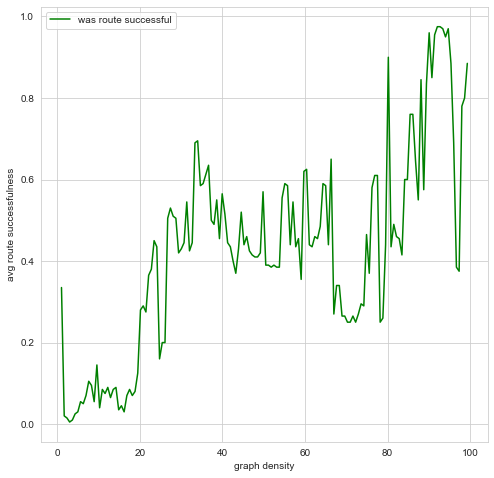
\includegraphics[width=8cm]{figures/random_uj/edge_den_succ.png}
  \hspace{1cm}
  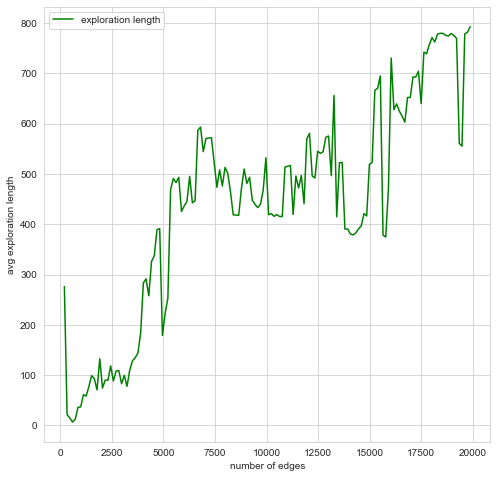
\includegraphics[width=8cm]{figures/random_uj/edge_expl.png}
  \vspace{1cm}

  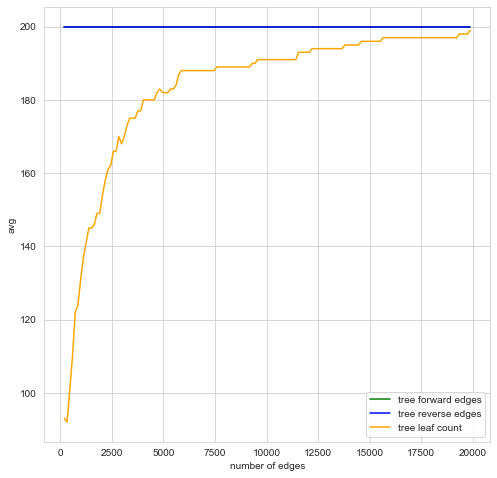
\includegraphics[width=8cm]{figures/random_uj/edge_tree.png}
  \hspace{1cm}
  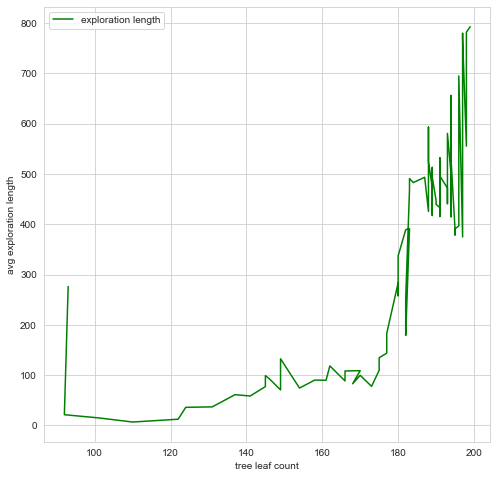
\includegraphics[width=8cm]{figures/random_uj/leaf_expl.png}
  \vspace{1cm}

  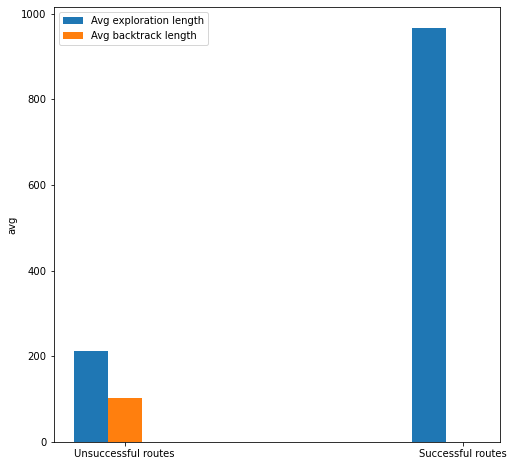
\includegraphics[width=8cm]{figures/random_uj/bar_plot_3.png}
  \hspace{1cm}
  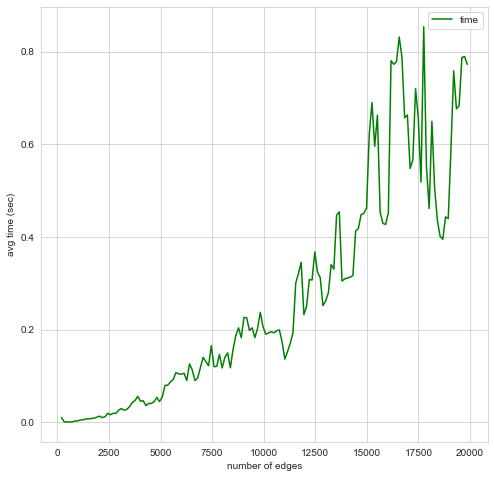
\includegraphics[width=8cm]{figures/random_uj/edge_time.png}

  \caption{Measurements on random graphs. All graphs have a fixed node count.}
  \label{fig:random-results}
\end{figure}

\begin{figure}
  \centering
  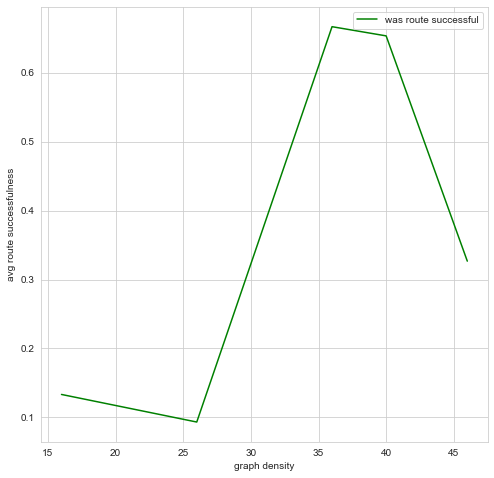
\includegraphics[width=8cm]{figures/reg_uj/edge_den_succ.png}
  \hspace{1cm}
  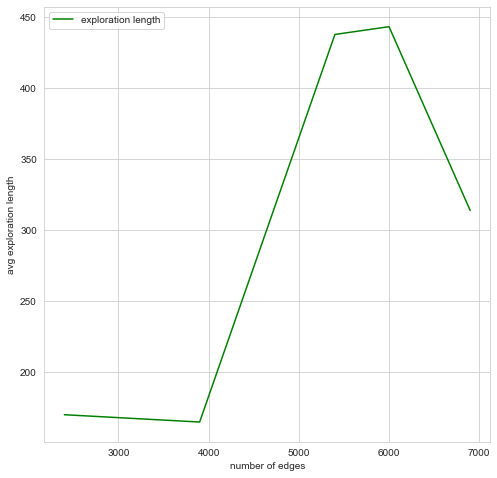
\includegraphics[width=8cm]{figures/reg_uj/edge_expl.png}
  \vspace{1cm}

  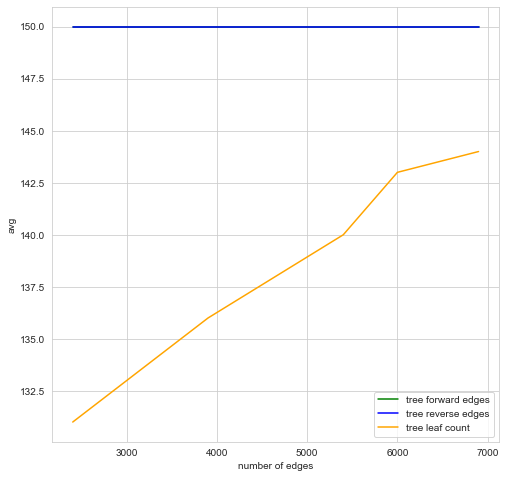
\includegraphics[width=8cm]{figures/reg_uj/edge_tree.png}
  \hspace{1cm}
  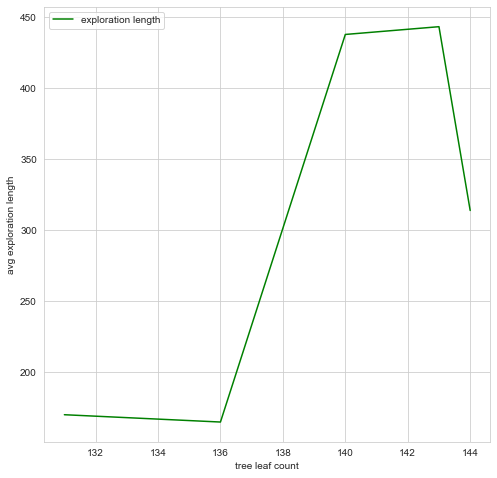
\includegraphics[width=8cm]{figures/reg_uj/leaf_expl.png}
  \vspace{1cm}

  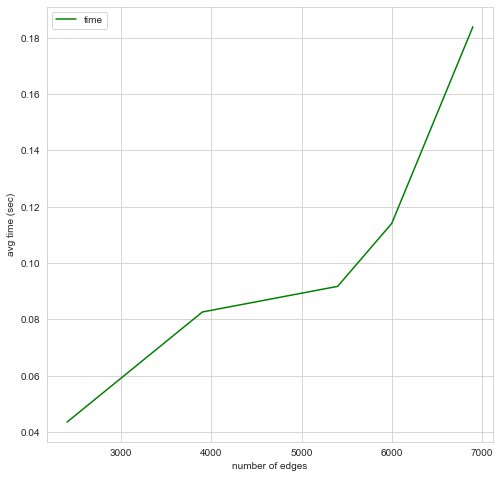
\includegraphics[width=8cm]{figures/reg_uj/edge_time.png}

  \caption{Measurements on regular graphs. All graphs have a fixed node count.}
  \label{fig:regular-results}
\end{figure}

% Turn on page numbering.
\pagenumbering{arabic}
\restoregeometry

\section{Future work}
\label{sec:future-work}

It remains to show or disprove that the ,,more regular'' a graph gets, the higher the success chance is for a route exploration. There are a number of challenges to overcome on that front; coming up with a sensible regular graph generator, and variants of that generator.

While we've shown a strong correlation in between edge density and success rates, we are curious whether the number of reverse edges in the spanning tree correlate even stronger. Indeed, what if some other metrics are those that really influence success rates? Further research could shed some more light on this.

We took a rather literal interpretation of the algorithm discussed in \cite{gorain2018deterministic}. Its likely that the robot could be smarter, for instance, knowing the routes that already failed, it could guess its location of its graph, or rule a number of nodes out. The oracle might be able to recognize special traits of a graph, like regularity. In that case, node count and degree would already be a sufficient advice; the robot could explore the corresponging universal traversal sequence.

\section{Conclusion}

We researched a novel approach to the graph traversal problem. In a connected, undirected, port numbered graph, we discussed how a robot could visit every node at least once with an outsides entity, called an oracle, supplying an advice. We focus on a case where said oracle -- called a map oracle -- is unaware of the starting position of the robot. The advice such an oracle can produce forces the robot to try, and occasionally failed to explore a number of routes.

We learned that the successful exploration of a route the robot constructs doesn't depend on the route's starting point having to be equal to the starting position of the robot. In fact, we learned that a great number of routes can lead to the full exploration of the graph. This motivated us to research what traits of the input graph or the advice might influence the rate of success on these explorations.

We showed that there is strong correlation in between the edge density of a graph and the route of success on the route epxloration. We further conjectured that regular graph, or graph with regular components migth also correlate with success rates.

\bibliographystyle{IEEEtran}
\bibliography{IEEEabrv,references}

\end{document}

